\documentclass{report}
\usepackage{graphicx} % Required for inserting images
\usepackage[italian]{babel}
\usepackage{tikz}
\usepackage{hyperref}
\usepackage{amsmath}
\usepackage{xcolor}
\usepackage{float}
\usepackage{soul}
\usepackage{listings} % Per evidenziare il codice

\definecolor{lightgray}{rgb}{0.9,0.9,0.9} % Definizione colore sfondo
\definecolor{darkgreen}{rgb}{0.0, 0.5, 0.0}

\lstset{
    backgroundcolor=\color{lightgray}, % Sfondo grigio
    basicstyle=\ttfamily, % Font monospaziato
    % frame=single, % Bordo attorno al codice
    tabsize=4, % Dimensione tabulazione
    breaklines=true, % Permette di andare a capo automaticamente
    numbers = left,
    numberstyle=\small\color{gray}
}

\title{\huge\textbf{{Security for A.I.}}}
\date{Parte III}

\begin{document}

\maketitle
\tableofcontents
\newpage

\chapter{STRIDE-AI}

\noindent Con \textit{Security for A.I.} si intende fare un \textit{threat modeling} per modelli di intelligenza artificiale; in questa lezione 
vediamo l'approccio STRIDE-AI.

\noindent STRIDE-AI vuole fornire una modalità strutturata per capire quali sono gli asset critici, per poi identificare quali sono i rispettivi 
failure mode e relativi threat. 

\begin{figure}[H]
    \centering
    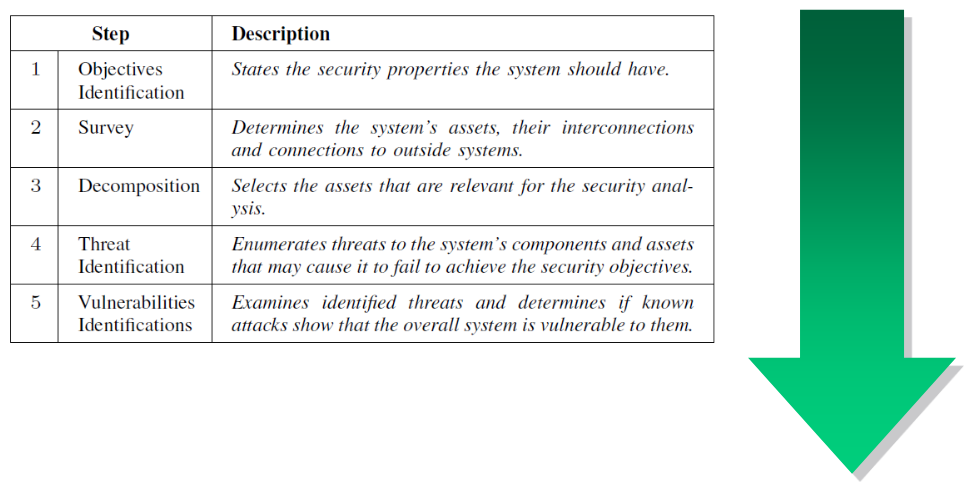
\includegraphics[width=1\linewidth]{images/threat-modeling.png}
    \caption{Processo di threat modeling}
\end{figure}

\begin{figure}[H]
    \centering
    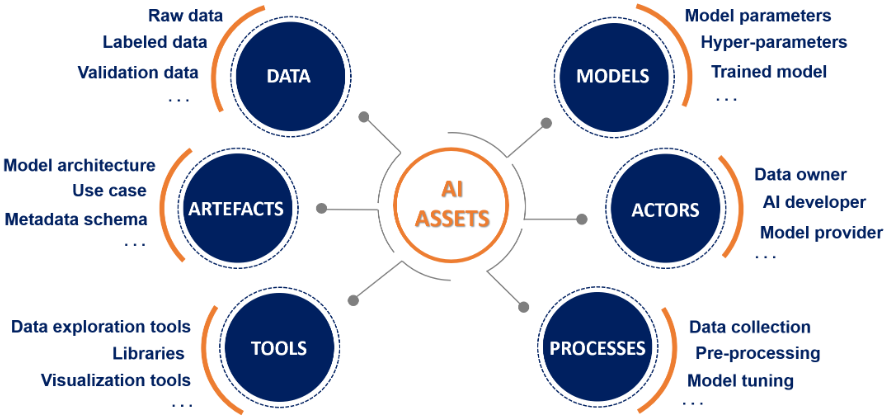
\includegraphics[width=1\linewidth]{images/ai-assets.png}
\end{figure}

\noindent STRIDE-AI prende i threat classici della metodologia STRIDE e li mappa in delle proprietà specifiche per modelli di intelligenza artificiale:

\begin{figure}[H]
    \centering
    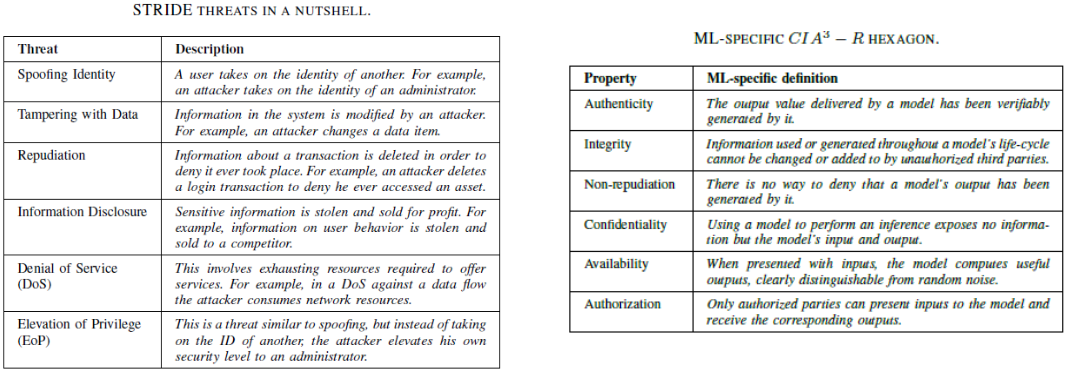
\includegraphics[width=1\linewidth]{images/mapping.png}
\end{figure}


\noindent Dunque, il processo che segue è:
\begin{itemize}
    \item fare un'analisi dell'architettura del sistema
    \item identificare quali sono gli asset 
    \item identificare quali sono i failure mode per ciascun asset 
    \item dai failure mode risalire a quali sono le proprietà di sicurezza che vengono negate
\end{itemize}

\noindent Ad ogni proprietà sono associati dei threat noti, e si possono applicare delle misure di sicurezza.



\chapter{Sicurezza di modelli ML contro attacchi di poisoning}

In questa lezione vediamo un framework di difesa contro attacchi di poisoning a modelli di 
machine learning.

\noindent Una delle assunzioni chiavi del machine learning è che un modello addestrato sui dati di training avrà una buona accuratezza e performerà 
bene dato che il training set è ben rappresentativo dei dati che il modello vedrà in fase di deploy\dots un training malevolo, dovuto 
ad esempio ad attacchi di poisoning, può mettere fuori uso un modello di machine learning.

\begin{figure}[H]
    \centering
    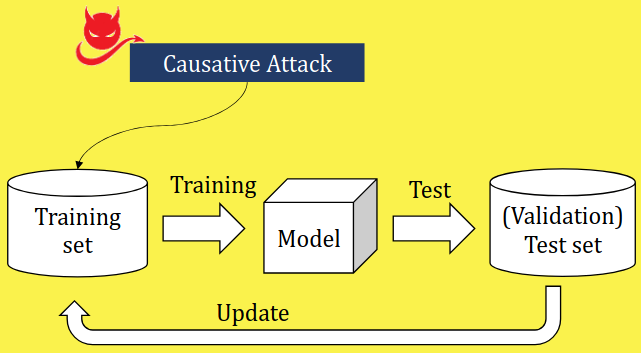
\includegraphics[width=0.7\linewidth]{images/poison.png}
\end{figure}

\noindent Alcune strategie di difesa contro attacchi ai dati di training sono:
\begin{itemize}
    \item \textbf{meccanismi di rilevamento} che mirano ad identificare i dati avvelenati e sanitificarli, oppure escludere 
    i dati sospetti (come gli outlier)
    \item \textbf{meccanismi di \textit{miglioramento}} che agiscono nella fase di addestramento cercando di impedire che possa avvenire 
    l'avvelenamento (ad esempio vengono introdotti dati avvelenati per ridurre la sensibilità ad un attacco)
    \item \textbf{model composition} che prevede di ridurre l'interferenza dei punti avvelenati tramite una suddivisione del training set 
\end{itemize}

\noindent Bisogna sempre considerare un trade-off tra accuratezza e robustezza di un modello di machine learning.

\subsubsection{Analisi del rischio dei data assets di un modello di ML}

\begin{itemize}
    \item Viene usato un classificatore \textit{Support Vector Machine} (ovvero un tipo di classificatore lineare) per stimare il rischio associato ai dati di addestramento
    \item L'idea è quella di mettere in relazione l'indice di rischio con la vicinanza dei punti ai SVM, ovvero lo superfici di separazione 
    delle classi
    \item L'attaccante usa una sua SVM per stilare quali sono secondo lui i punti più a rischio, e decidere in quale direzione fare una modifica
    \item Il risultato è ottenere delle partizioni del training set che vengono utilizzate per addestrare dei sottomodelli, che saranno poi combinati tra 
    loro per ottenre il risultato finale
\end{itemize}

\begin{figure}[H]
    \centering
    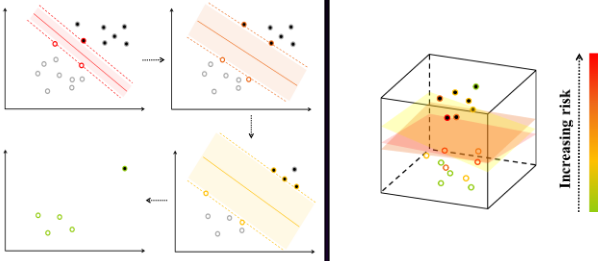
\includegraphics[width=0.8\linewidth]{images/svm.png}
\end{figure}

\noindent La strategia prevede di usare l'\textit{anti-clustering} per ottenere delle partizioni con una massima diversità interna e una 
minima diversità tra i gruppi; in particolare, si prevede che punti vicini con alti livelli di rischio siano distribuiti in partizioni 
diverse, in modo da ridurre il rischio di compromettere più sottomodelli. 

\noindent Possiamo quindi dire che:
\begin{itemize}
    \item suddividendo oppurtanamente i dati e combinando le predizioni dei modelli, \textbf{gli errori sui dati risultano indipendenti tra loro}, garantendo così robustezza 
    \item segue che un \textbf{numero sufficiente di sottomodelli intatti} garantisce che il risultato finale non sia corrotto.
\end{itemize}














\end{document}
